%%%%%%%%%%%%%%%%%%%%%%%%%%%%%%%%%%%%%%%%%%%%%%%%%%%%%%%%%%%%%%%%%%%%%%%%%%%%%%%%%%%%%%%%%%%%%%%%%%%%%%
%
%   Filename    : chapter_3.tex 
%
%   Description : This file will contain your Theoretical Framework.
%                 
%%%%%%%%%%%%%%%%%%%%%%%%%%%%%%%%%%%%%%%%%%%%%%%%%%%%%%%%%%%%%%%%%%%%%%%%%%%%%%%%%%%%%%%%%%%%%%%%%%%%%%

% Please refer to the following resources regarding Theoretical Framework: 

% \begin{itemize}

% \item \url{https://link.springer.com/chapter/10.1007/978-1-4419-1454-5_12}
% \item \url{https://link.springer.com/article/10.1007/s10972-015-9443-2}



% \end{itemize}



\chapter{Theoretical Framework}

This chapter provides a clear discussion of different studies and theories
behind each concept of the study. 
The first section will discuss the theories on Human-Computer Interaction, Interaction Design and also Evaluation methods on User Experience, while the last section will focus on Musical Representation. These will be accompanied on the other hand with theories on how children go about in these respective ideas.

\section{Interaction Design} 
Interaction design as described by \citeA{PreeceRogersSharp15} is \say{designing interactive products to support people in their everyday and working lives}, that helps in creating a user experience that enables the users in their work and interaction with others. People use interactive objects everyday like phones, machines, etc., but not all of these are easy to use or effortless. Interaction design focuses not only about giving people a product but also how it understands how a particular feature can affect how people work as well as how it can improve their experience \cite{dix2009human,PreeceRogersSharp15}.

The aim of interaction design is to integrate usability in designing the system, that makes a product that is easy, effective, and enjoyable to use for the user \cite{PreeceRogersSharp15}. User satisfaction is of vital importance in interaction design.The further study of interaction design have led to experts creating processes and identify a group of design principles. These principles will serve as a help in creating good interfaces for users \cite{PreeceRogersSharp15}.

The use of interaction design will be integrated in the different iterations of designing the application. This theory will be important in identifying the principles that will serve as our guidelines in designing the interactions in the interface.

%Children interaction design
%
%Despite the young age of the field of interaction design for children, There are some basic principles that have been developed by researchers over the years \cite{hourcade2008interaction}. 

%Visual Design
%The important aspects of visual design for the children are the icons, text and the complexity. For humans in general, Icons must be easy to to recognize that it can be interacted, represent what they do properly and are distinguishable from each other. The only difference for children is the size of these icons must be proper for the children. The text has to have minimized usage unless it is an application to teach reading. Finally, the visual complexity of the applications must follow multi-layer strategies. These are strategies where children are presented with a few actions or icons to interact with at first and are presented with more as they progress. 

%Interaction Styles
%There are three main interaction styles. The first being the usage of direct manipulation. The main ideas that direct manipulation utilize include visibility of objects and actions of interest. The visibility of objects and actions of interest involve making objects have distinct look that shows there are actions that can be done to them.

%The actions for the objects must be rapid, reversible, and incremental. The actions must be rapid because children tend to be less patient than adults. If the children do not get quick feedback from the action they are likely to lose interest. If an action cannot be rapid, children must still have some way of knowing the status of an action (such as progress bars), the children must be still able to interact with application in another way during the other action taking place and the children must have an option to cancel the action. Reversibility, meaning actions can be undone, on the other hand encourages children exploration while making them remain in control. An action of resulting in a loss of child's creation might lead to frustration and the child losing the desire to use the application anymore. Finally the need for an incremental actions, meaning step by step actions, is required so children can do complex tasks. Without these incremental actions, children may find themselves stuck in a task and unable to progress due to solution being to complex leading to frustration. 

%Another interaction style is the menu. Children are almost always presented with a menu since even a set of choices can be considered a menu. The problem with menus however comes when choices are not immediately visible such as drop down menus. It is found out that menus that had to be brought up with a were easy to forget especially for children making it confusing for them.

%The last interaction style is text based interaction. This becomes a problem when children need to type for them to interact with a computer but do not know how to type yet. Similar to lack of the lack of ability to type is the lack of knowledge to spell. A problem would arise if  commands need proper spelling but the child is unable to spell them correctly. These interactions may significantly slow down as the child lacks the ability to do them.
%

\subsection{Human-Computer Interaction}
Human-Computer Interaction or also known as (HCI) studies ways on how many different computer technologies affect human activities \cite{dix2009human} and how it enhances the quality of interaction between humans and the computer \cite{baecker2014readings}. Research in this field has been an integral part in the development of early systems, like the graphical interface of Windows 95 and another is that it has greatly improved the World-Wide Web \cite{myers1998brief}. Both these early systems show how HCI research has greatly improved the usability of their system and how further interface improvements has enabled more research to be done on this field. 

\citeauthor{kaptelinin1996activity} characterized the subject Human-Computer Interaction in three dimensions as seen in figure \ref{fig:three_dimensions}. The first is the interaction between the user and the environment which transcends the user interface, it explains how the interaction with computers help people in achieving their goals. Next is development, and he describes this as the user develops from being a novice to often becoming an expert. Last is the individual/social dimension as he characterized the word \say{user} not only as an individual but also as a group or an organization.

\begin{figure}[H]
    \centering
    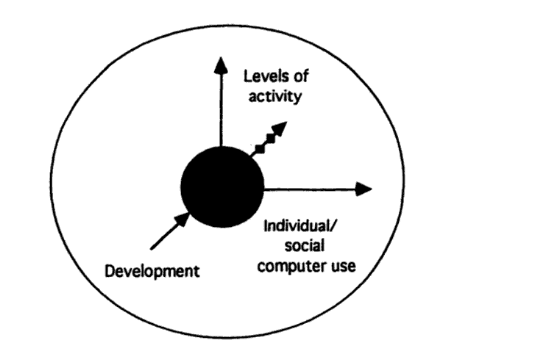
\includegraphics[width=12cm ]{figures/three-dimensions.PNG}
    \caption{HCI Three-Dimensions \protect\cite{kaptelinin1996activity}}
    \label{fig:three_dimensions}
\end{figure}

According to \citeA{inbook}, one of the core topics of studying HCI is the usability of these technologies. Usability according to \citeA{frokjaer2000measuring} is described as taking into three different aspects such as satisfaction, efficiency, and effectiveness. Satisfaction takes into account the use of the system and how comfortable they are with it \citeA{frokjaer2000measuring}. Also described by \citeA{frokjaer2000measuring}, user satisfaction is described as the preferences of the user on the usage of the application on the tasks given to them. Efficiency talks about the relation between users completing the tasks and the resources used to do it \cite{frokjaer2000measuring}. Lastly, effectiveness shows how users properly do their tasks and also achieve certain goals in using the system as determined by some indicators of efficiency for example the completion time of tasks and learning time \cite{frokjaer2000measuring}.

The increase of research in this field as well as the emergence of better technologies has led to the creation of new topics under Human-Computer Interaction like studies on interaction design and user experience.

\subsection{Mobile Interaction Design} 
Interaction Design can also be applied to mobile applications like smartphones and tablets. The change of integrating an application to a mobile platform presents unique challenges in making the interaction. According to \citeA{tidwell2010designing}, these challenges can be summarized into 5 categories. (see Table \ref{Challenges}).

\begin{table}[H]
\centering
\caption{Challenges of Mobile Design} \vspace{0.25em}
\begin{tabular}{|l|l|} 
\hline
\textbf{Challenge}                                                         & \textbf{Description}  \\ 
\hline
Tiny Screen Sizes                                                          & \begin{tabular}[c]{@{}l@{}}In mobile devices space for information is limited. Unlike \\in computers where there are long header menus, in desi-\\igning a mobile application all the excess~assets should be \\removed \cite{tidwell2010designing}.~ ~ ~~\end{tabular}  \\ 
\hline
\begin{tabular}[c]{@{}l@{}}Variable Screen~\\Widths\end{tabular}           & \begin{tabular}[c]{@{}l@{}}The second challenge presents the difficulty in making a~\\design that would scale well on different screen sizes ~\\ \cite{tidwell2010designing}.\end{tabular}                                                                                   \\ 
\hline
Difficultly of Typing                                                      & \begin{tabular}[c]{@{}l@{}}Users do not like it when there is a need to type large am-\\ounts of ext with the keypad \cite{tidwell2010designing}.\end{tabular}                                                                                                           \\ 
\hline
\begin{tabular}[c]{@{}l@{}}Challenging Physical\\Environments\end{tabular} & \begin{tabular}[c]{@{}l@{}}Lastly, people use their mobile devices in different places.\\Places where it could be really bright or dark, during tran-\\sportation, in bed, etc.\cite{tidwell2010designing}.\end{tabular}  \\
\hline
\end{tabular}
\label{Challenges}
\end{table}

For our application the other problems are not to be tackled as much, as firstly the problem on variable screen widths is as not a problem since we will only focus the iPad. Second, the difficultly of typing is not much of a problem since the user will not type a huge amount of text. Third, the environment where the child will use this is not a problem since the place will mostly be indoors. For the application, we will mainly focus on the problems of tiny screen sizes and touch screens seen in Table \ref{Challenges}. The problem of tiny screen sizes in our application is that the size of the iPad screen would be limited as we would also have to properly put the assets on the screen to minimize this. Lastly, the problem on touch screens is what this study aims to solve as we would use gestures aimed to help the interaction between the interface and the user's fingers.

\subsection{Design Principles}
These principles are used in solving the challenges provided in designing the interaction for the users. \citeA{blair2008user} described design principles as \say{clear rules of thumb} that also consist of defined features, \citeA{kimball2013visual} also described that these principles are heuristic methods that help in making decisions. \citeA{norman1999affordance} also states that a successful design comes with a set of underlying principles.  

In making systems developers and companies often think that they should only focus on enhancing the aesthetic appearance of their product in itself rather than also putting equal importance with the overall experience and usability of them \cite{norman1999affordance,blasing2010android,stephanidis2012encyclopedia}. Having a clear idea of the goal of the software from the start is very important, as the interface can be made to achieve the goal that was set and the design should highlight what the goal is \cite{blair2008user}. The overall goal is to design a product that is pleasing to the user for both viewing and using.

\citeA{williams2015non} and \citeA{stephanidis2012encyclopedia} both state four key principles to acknowledge in designing interfaces for different kinds of platforms. The first is \textit{contrast}, this makes the use of shapes, colors, and sizes to draw the users attention. Following this makes it easy for the users to distinguish where they need to focus on. Second, is \textit{repetition}, it talks about having a consistent visual scheme that it makes it easier for the users to recognize. The use of same text, colors, and fonts helps in unifying the design. The third is \textit{alignment}, and this principle talks about the placement of the design elements through out each screen in the system. This principle brings order to each screen and makes the design much more uniform to one another. Last is \textit{proximity}, this principle brings related design elements to be grouped together to show how each element is connected and helps in focusing the users attention. 

Other important principles on the other hand are suggested by \citeA{blair2008user}, one of them is the principle of an Obvious Starting point. This principle can also be used because the user needs to know how to start interacting with the system. The starting point can serve as the point where the user learns more about the interface from the first encounter and cognitively finding patterns helps in the learning. Another is a Clear Reverse and this principle explains how the user can obviously see the way to reverse a particular action or exit the session. Knowing a way to reverse an action or having a clear exit route may give users a sense of confidence in using the system as they need to experience that they can experiment with the system without damaging it.

%Mobile Design Principles
Mobile interfaces have there own limitations when compared to the normal setting of desktop interfaces \cite{gong2004guidelines}. Due to these limitations design principles that are used for desktop interfaces have been modified to aid in creation of mobile interfaces \cite{gong2004guidelines}. \citeA{nilsson2009design} suggests guidelines that help in answering some common issues in mobile interfaces found in Table \ref{Challenges}.

For the problem of screen space an issue identified was the issue of horizontal scrolling this is due to the fact that information on the screen is usually more connected to ones in the same line rather than the ones in different lines \cite{nilsson2009design}. The principle provided to answer this issue is for the attributes on the screen is to be optimized in terms of size and sequence. Changing the layout can help in avoiding the need of horizontal scrolling, an example is changing the screen orientation if the user is given an option to change between landscape and portrait or only given one of the two \cite{nilsson2009design}. Another problem is in typing text, as the keyboard that is provided is usually small for the users that it is hard for the fingers to enter \cite{nilsson2009design}. The principle provided to answer is to provide auto complete of text by trying to predict the word the user is typing by giving suggestions near the current type letters. The last problem is in touch screens, as not all mobile devices are given a stylus that helps with the users interaction with the device. A Principle to help solve this issue is to make the menu choices finger friendly, since the problem lies on the fingers not always hitting the small details of the screen making interaction mechanisms like lists, buttons, menus, etc. finger friendly helps the use in having more control in the application \cite{nilsson2009design}.   

Though the principles presented are not solid rules, nonetheless these principles can still be heavily considered in being followed when designing an interface. The principles mentioned in this subsection will be used as a guide in designing the interface. The four key principles will be taken into consideration in the designing of the assets in the sandbox environment and also in the flow of the usage of the application. We will use the principle of the obvious starting point so that the child will have a screen that they can go back when they are lost. For the clear reverse this is very helpful as the child will make mistakes in using the sandbox and this is helpful so that these mistakes are reversed to let the child finish their tasks. 

\subsection{Gestural Interaction}
The goal of Human Computer Interaction is for humans to naturally interact with technologies like computers for their everyday use \cite{hasan2012human,rautaray2015vision}. For a long time gestures have been considered as a bridge for the humans to interact with these computers, because of the popularity in the usage of hand-held touch screen devices like smart phones and tablets \cite{ruiz2011user,hasan2012human}.

According to a study by \citeA{roth2001gestures}, gestures can be characterized into four. First is \textit{Rest} that actions begin from the point of rest, then it moves away to another position and eventually return to the point of rest. Second characteristic is \textit{Peak or Stroke}, which shows the moment of the gesture which denotes movement. The third is the \textit{Preparation and Recovery Phase}, is when the hand goes back to the resting position. Last is that usually gestures are \textit{Symmetrical}.

There are many user interfaces that gestural interactions have been considered very natural, yet others are harder to understand at first like the multi-touch gestures for devices like tablets compared to other gestures where it can be easily be learned by the user \cite{mortensen_2019}. An example for mobile device users is the simple gesture of swiping left or right compared to a more complex gesture like a multi-finger swipe in a certain direction \cite{mortensen_2019}.

Touch gestures have been seen as an intuitive way of communication between the user and the computer, the actions that build up specific functions makes it natural to use \cite{rautaray2015vision}. In a research done by \citeA{chan2019applying} tasks were made possible with the use of gestures. In integrating the gestures for their mobile musical composition tool they recommended 5 gestures that can be used for similar tasks, these gestures are Tap, Tap & Hold, 1-Finger drag, 2-Finger drag and Pinch. In the different iterations of their research they were able to map the appropriate gestures to accommodate the tasks needed for their composition tool.  

%Children mobile interaction design
%Mobile interaction design gestures.
There are many gestures for mobile applications that use a touch screen. Common gestures include tapping, flicking, sliding, dragging & dropping, rotating, pinching and spreading \cite{aziz2013children}. Generally younger children that are below age 4 may have a hard time with some gestures due to not being familiar with them. Children above age 4 however know how to use all these gestures. Specifically children aged 7-12, have no problem using these gestures to deal with 2D or 3D objects. They do not even have problems doing different gestures in a single application or interface. However they seem to prefer apps that focus on tapping. These children as well prefer more fun and more challenging applications to keep their attention.

For the gestures of the application we will be following the research of \citeA{chan2019applying} as they already provided specific gestures that can be used in a musical application. In the integration of these gestures we would be focusing on how each gesture will help the user in completing their tasks. The specific gestures we would will be focused on the Tap, Tap & Hold and 1-finger drag. For the Tap this gesture will be mostly used in the buttons. The Tap & Hold will be used as a preview of the parts of the firefly model. Lastly the 1-finger drag will be mostly used on assets regarding adjustments and scrolling.

\subsection{Gestalt Principles}
The set of Gestalt Principles comes from psychology, where it says how the human brain will simplify things like elements and recognizing patterns. The Gestalt principles provide six fundamental laws that designers can follow \cite{yee2002user,chapman_2018}.

\begin{enumerate} 
\item Figure/ground
\item Similarity
\item Emergence
\item Closure
\item Continuation
\item Symmetry and Order
\end{enumerate}

\textit{Figure/ground} explains the distinction of the object with relation to the foreground and background of the design.The important thing in this law is how it contrasts and how the object is still visible and understood.

\textit{Similarity} says that humans usually see the same things like size, color, or shape in the design of elements and they tend to group them together. The main use of similarity is to bind elements together that are not necessarily next to each other in the design.

\textit{Emergence} shows how elements that are in range of each other can be grouped together while others also near one another are grouped separately.

\textit{Closure} explains how humans want to see complete objects so if they don't they visually connect missing information through familiarity and patterns seen.

\textit{Continuation} talks about how the human eye will most likely follow a smooth path and it would want to see a clear flow of these visual elements.

\textit{Symmetry and Order} takes into consideration how the design is complete and balanced, because if not time and effort will be exerted by the user in trying to understand it.

The gestalt principles will be used in the application to help design the different parts of the screen. All of these will be taken into consideration but some would be used more, as some assets need these specific principles to be displayed much clearer. In designing the objects in the interface the figure/ground principle helps us in distinguishing these objects from the background so it can be clearly seen by the child. We will use the Similarity principle in designing assets in screen as our target users which are children need to identify visual patterns to be able to complete their tasks. The principle of Emergence will be used in grouping similar assets together to make it easier for the child to identify their functionality. Lastly Symmetry and Order helps us in making the application much more balanced to help the child immediately understand the functionality of the system.

\section{Understanding Children Interaction}
As HCI maybe generally for understanding general humans, we need to focus on children as they have aspects adults do not have. These aspects can result in them having different needs compared to usual adults to where HCI is generally designed for. 

\subsection{CHI Techniques Enabled Through Play}
%CHI PLAY
 CHI Play is a yearly conference that focuses on topics across all areas of play, games and human-computer interaction. They feature papers that show different techniques and practices for games. Some of these are specifically studies are aimed towards children and we can use them for designing our application.

A study by \citeA{gray2018designing} analyzes five commercially available applications for preschool children. They discuss what factors in these applications may lead to children liking or disliking the application. They discuss the importance of characters, support for competence, interaction complexities, and the understanding of buttons and menus. Different game characters with different personalities may increase the chances of a child liking a character which would contribute to the game's enjoyment. Support for competence involves a child getting in-game rewards for doing good in the game. This may increase enjoyment as the children enjoy sharing their achievements however giving the child negative feedback upon doing badly in a game lessens enjoyment as well. Interaction complexities described that confusing tutorials such as one where actual game play cannot be differentiated from a tutorial makes it confusing for the child. This makes them think they were doing things right but it was just the tutorial auto playing for them leading them to perform badly when it came to the actual game. Understanding buttons and menus talk about the difficulty of children have with complex menus and how they ignore text based interaction. They also seem to not understand some symbols and colors of the buttons but can find out what they do with game play. 

A study by \citeA{scheepmaker2018things} discusses that play has a different definition for children as it does for adults. For adults it is generally any enjoyable activity however for children it is something they want to and get to do. Specifically, the children are in control meaning they started playing because they want to. This means they play for them includes things that they do not need to finish or seek approval. An important aspect of play is called appropriation. Playful appropriation is a transformation of situations or elements into fun experiences. An example seen in the paper involved an animal like robot designed to bring out certain behaviors in children. The different children had different abilities and experiences therefor leading to them having different ways to appropriate the robot into their own versions of play. This leads to the idea of designing applications for appropriation. These designs are defined to be ambiguous,in need of a user who will complete them and break away from a usual designer-centered thinking where the system makes it clear how the system should be interacted with. 

A study by \citeA{li2018understanding} shows talks about playfulness. In general, it is a mindset where something is approached without seriousness or a clear goal. Playfulness may help in making products go beyond their initial level of entertainment. An idea for interaction for a play setting is described by \citeA{crowell2018role}. This idea discusses interaction for play is a three stage model. The three stages are invitation, exploration and immersion. Invitation is the state where the system should invite the user to engage with it. Exploration is when the user is trying out different possibilities with the system. Finally immersion happens when the user has explored enough with the system and is creating different things that applies everything learned in the exploration stage.

FireflyX would be able to use support for competence in order to motivate the children in the first paper by \citeA{gray2018designing}. This can be seen at the very least in the tutorial when the children is congratulated for completing it. It would be also be able to use interaction complexities for its tutorial and use understanding of buttons and menus for the design of the user interface. This can be used specifically used by making objects that can be interacted appear differently from objects that cannot be interacted with. For the second paper by \citeA{scheepmaker2018things}, FireflyX can use definition of play and try not to use the usual design centered thinking in its design. By this, we will design FireflyX in a way that children will discover different ways how to use an application and the app will not have a single way to use it. In the last works by \citeA{li2018understanding} and \citeA{crowell2018role}, FireflyX can use these three stages in its design and work around it. For the first stage, we can invite children to interact with objects with obvious signs such as glowing and moving objects. In the second stage, the app must be designed in a way that a child can explore the different possibilities of its uses without being limited. This can be helped done by having a minimum tutorial to show the bare minimum of what a child needs to know in order to use the app. Another way to apply this is also not having objectives or just having a few that so that the child's mentality does not focus on achieving them and are free to do whatever they want. 

\subsection{Theories on Children's Cognitive Development}

Aside from papers from the CHI PLAY conferences, there are also general theories associated with children's cognitive development. Due to how children today are reported to have an increased used on computers, it is important to take into account the children's interests, abilities and developmental needs in the design of these technologies \cite{hourcade2008interaction}.

In order to maximize the learning of the children, existing research on child development must be considered. Jean Piaget, one of the most influential experts on child development, has views on children that have affected the field of computer child interaction. Three of his works are to be considered for computer child interaction. The first work talks about how children construct knowledge. The second work talks about the factors that affect development and finally the last work talks about the different developmental stages children go through \cite{hourcade2015child}.

Piaget observes that learning occurs during a process of adaptation. When children are undergoing adaptation, they are creating their own knowledge when they are experiencing and interacting with the world. However the idea that children make their own new knowledge from their experiences and their own current existing knowledge is called constructivism. However, Seymour Papert a Key figure in child computer interaction expands on Piaget's ideas and proposes constructionism. This proposal talks about how adaption works best when children are making something to share with others. This emphasizes on providing children technologies where they get to be creators. This proposal puts an emphasis on social and motivational aspects of learning as well as providing children more opportunities to alter modify their environment.

Piaget discusses that there are four aspects that affect development. These are maturation, experience, social aspects and emotions. Children's physical maturation limits their learning. The limited cognitive and motor abilities of children affected by their maturation would limit their interaction with technology. On the other hand, experience is a important factor for adaptation as it is required in the building of knowledge. This puts emphasis on experiencing the world rather than being told by it. These unique experiences can be be provided or augmented with technologies using virtual environments or simulations. Social aspects such as social interaction play a key role in development such as when children copy the way of how experienced adults complete think and complete tasks. Technologies can help in this field by linking ideas and interests for children and the experienced adults. With the thought of emotions comes motivation. Motivation affects development since it deals with the children's drive to grow. It can be achieved by making learning relevant to children's lives and interests. Papers expands upon this by believing that learning activities with topics that children are passionate about will motivate learning better. This highlights the need for flexible learning activities that answer to every child's interests. This is where computers can shine due to their ability to provide a variety of learning activities and opportunities. Commonly used software to provide a variety of learning today are games.

Piaget proposes four stages of development: the sensory-motor stage, pre-operational stage, the concrete operations stage, and the formal operations stage. We will only discuss the pre-operational stage and the concrete operations stage because that is where our target audience lies. Children ages 2 to 7 are included in the pre-operational stage and are focused on seeing the world on their own perspective. This makes them usually focus on one object at a time which limits understanding navigation through hierarchies. The concrete operations stage include children age 7 to 11. These children are more likely to appreciate another one's perspective making them suitable as design partners with adults for making applications. Due to this, they are also able to understand hierarchies and are compatible with more types of technology.

Another theory for cognitive development are the information processing theories. These theories treat the brain as a computer that manipulates information. Cognitive task output is affected by changes in the information in the mind and mental hardware as the brain develops. For children, this often leads to variability in their cognitive tasks, in which children are choosing from an array of strategies and will not stick with the same strategy consistently. As time passes, they may end up preferring the most successful strategy for them though another cause for variability is trying to apply the same strategy towards a variety of tasks having different results in success. Children's variability must be taken into account in usability testing with them.

From these theories, we can use the theories by Piaget in designing FireflyX as it mentions to avoid the use of navigation through hierarchies such as drop down menus and motivating children by making activities relevant to their interests. Other ways we can apply the theory also include by knowing what children have learned and experienced in their schools in our age target, we can know what they are capable of understanding and adapting to. The information processing theory can be used to see if repetition is effective during observing as it mentions variability to which children try different things in doing the same tasks until they are successful. By seeing a child try different things in different attempts to achieve the same thing, we can say that repetition of the same task for learning is useful. As also mentioned by Piaget, trying out new ways to achieve something may also be form of adapting which enforces repetition as kind of a form of forcing adaptation on the child. 


%\subsection{Bloom's Taxonomy}

%While theories can help understand development, there is also a concept that aids in development. In schools, a concept known as a Bloom's Taxonomy can be used to design their curriculum \cite{krathwohl2002revision}. This concept shows the different cognitive processes important for learning which serves as the basis for the curriculum schools have. The 6 main processes presented in this concept are remembering, understanding, apply, analyze, evaluate and create.

%The remembering process includes the ability to also recognize and recall. It is for people to retrieve knowledge from their memory on important topics. The next process which is the understanding process includes different abilities such as interpreting and explaining. It is for people to determine the message given by different forms of communication such as oral and graphic communication. Thirdly the applying process includes the abilities to implement and execute. It carries out procedural solutions towards different situations. Analyzing includes skills such as the differentiating and attributing. It is for people to be able to show how a material or process can be divided into different parts and how they relate to each other. Next comes evaluating which includes skills such as critiquing /checking. It gives people the ability to make decisions/judgement based on criteria and standards. Finally comes creating which includes skills such as planning and producing. This is for people to put materials/ideas together and make an original creation. Learning through these processes ensure the children are actually able to apply what they learned.

\subsection{Standards in Children Interaction Design}

To help with interaction, standards on how to design applications for children have been made. A study by \cite{markopoulos2003interaction} mentions that there are two major areas where designs should focus on. These areas are age specific interaction styles and the involvement of children in the design process. Age specific interaction styles include different interface related design such fonts, menu structures, on-screen object sizes, etc. The involvement of children in the design process can be showed in (to be added figure). In this figure, the relation of technology to children can start from children being end-users to children being designers. Moving from within the figure to the other layers to figure, children can become more active and responsible as well as being more involved in the design process.

However, the activities children do with technology are mostly limited to either education or play. Studies have explored the relationship between education and play \cite{markopoulos2003interaction}. These studies show that fun contributes as motivation for doing activities so utilizing it can make learning more effective. Playful learning is described to have five core elements. These elements are exploration through interaction; engagement; reflection; imagination, creativity, and thinking at different levels of abstraction and; collaboration.

Child computer interaction (CCI) is a relatively new research area which is defined with the same idea as a HCI but for children instead of humans in general \cite{read2011nature}. The necessity for CCI was associated with three main differences between children and adults with the use of computers which are activities, behavior and concern. Children do different activities with computers, behave differently around computers and have different concerns for computers when generally compared to adults. CCI has established provided 10 guidelines on how and what to design technology for children known as the 10 pillars of CCI \cite{hourcade2015child}.

\begin{enumerate} 
\item Work in interdisciplinary teams
\item Deeply engage with stakeholders
\item Evaluate impact over time
\item Design the ecology, not just the technology
\item Make it practical for children’s reality
\item Personalize
\item Be mindful of skill hierarchies
\item Support creativity
\item Augment human connections
\item Enable open-ended, physical play
\end{enumerate}

\textit{Work in interdisciplinary teams} talks about how teams should be composed of people experience in design and evaluation methods for the technology builders (computer scientists, etc) and experts at the target children population (teachers, parents, etc.). Optionally a team may also have a designer and a expert on the topic where the technology covers (librarian for library software).

\textit{Deeply engage with stakeholders} talks about how every different generation of children has their own view, expectations, and experience with technology. As adults have difficulty remembering what it takes to be a children, they have to involve children in the design process in order to improve the chances of successfully making a child-centered design.  Even Adults that children interact with are also affected by these technologies so they also must have a role in the design process. If the design team isn't familiar with the stakeholders, they should interact with them more.

\textit{Evaluate impact over time} shows that children do not instant change as they use technology. They must be observed for an extended period of time to evaluate how technology has affected them. These changes include the children learning new abilities and skills.

\textit{Design the ecology, not just the technology} means the design process should not stop at the technology but must also be used in designing the physical environment. The people present when the technology is used and support activities can also be taken into account for designing the children's ecology when using the technology.

\textit{Make it practical for children’s reality} includes how designs should consider the context where the children may use the technology and if they are fit for the situations to be used in in order to be successful. Technologies should be relevant to children’s lives, needs, and interests.

\textit{Personalize} mentions that different children have different experiences, needs, interests, skills and more. Some children even come with specific impairments.  With these differences, personalization can provide great benefits in making technology advantageous for children.

\textit{Be mindful of skill hierarchies} talks about how in many fields, the learning process teachers basic skills before teaching its more complex skills where basic skills are needed.Design teams should take into account the basic skills needed for their interactive technologies. Skill hierarchies where the order of the skills to be learned should be taken note of.

\textit{Support creativity} takes place if learning is more motivating to the child if it done with a purposeful meaning such as in building. This is an application of the idea comes that from Seymour's idea of constructionism which again talks about how adaption works best when children are making something to share with others.

\textit{Augment human connections} is when technology doesn't interfere with a child's personal connections with primary caretakers and instead augment them can result in more positive development. Face to face interaction is a critical element in learning some skills such as negotiating, listening, sharing, etc. 

\textit{Enable open-ended, physical play} such as open-ended physical play is when children can play freely and creatively without limit. This can result in positive effects such as the child developing problem solving skills, having better health, learning to  engage with peers, etc.

Aside from these pillars ,there are also some basic principles that have been developed by researchers over the years \cite{hourcade2008interaction}. The important aspects of visual design for the children are the icons, text and the complexity. For humans in general, Icons must be easy to to recognize that it can be interacted, represent what they do properly and are distinguishable from each other. The only difference for children is the size of these icons must be proper for the children. The text has to have minimized usage unless it is an application to teach reading. Finally, the visual complexity of the applications must follow multi-layer strategies. These are strategies where children are presented with a few actions or icons to interact with at first and are presented with more as they progress. 

There are three main interaction styles. The first being the usage of direct manipulation. The main ideas that direct manipulation utilize include visibility of objects and actions of interest. The visibility of objects and actions of interest involve making objects have distinct look that shows there are actions that can be done to them.

The actions for the objects must be rapid, reversible, and incremental. The actions must be rapid because children tend to be less patient than adults. If the children do not get quick feedback from the action they are likely to lose interest. If an action cannot be rapid, children must still have some way of knowing the status of an action (such as progress bars), the children must be still able to interact with application in another way during the other action taking place and the children must have an option to cancel the action. Reversibility, meaning actions can be undone, on the other hand encourages children exploration while making them remain in control. An action of resulting in a loss of child's creation might lead to frustration and the child losing the desire to use the application anymore. Finally the need for an incremental actions, meaning step by step actions, is required so children can do complex tasks. Without these incremental actions, children may find themselves stuck in a task and unable to progress due to solution being to complex leading to frustration. 

Another interaction style is the menu. Children are almost always presented with a menu since even a set of choices can be considered a menu. The problem with menus however comes when choices are not immediately visible such as drop down menus. It is found out that menus that had to be brought up with a were easy to forget especially for children making it confusing for them.

The last interaction style is text based interaction. This becomes a problem when children need to type for them to interact with a computer but do not know how to type yet. Similar to lack of the lack of ability to type is the lack of knowledge to spell. A problem would arise if  commands need proper spelling but the child is unable to spell them correctly. These interactions may significantly slow down as the child lacks the ability to do them.

From the pillars, most of them can be used in the design of FireflyX due to its nature of being an educational sandbox for children. Deeply engage with the stakeholders pillars are done first so we understand what we need to create first which is what we get by talking to music experts. Work in interdisciplinary teams is not used because there are no real experts in the field of music in our team but we are discussing with the stakeholders to make up for that. Due to it being a sandbox, the pillars of support creativity and enable open ended play are applied as it is needed for children to explore and create different possibilities with the fireflies. Evaluate impact over time, Make it practical for children’s reality, Personalize and Be mindful of skill hierarchies need to be done since we are designing specifically for children in order for them to learn music so we must know what their skills and experiences for their age group is in music. Finally, Augment human connections and Design the ecology, not just the technology may not be used as this application might be standalone and does not need a supervisor and serve as a supplementary way for learning music .

The interaction styles that were mentioned can all also be used in the design of FireflyX to make it more child-friendly except of course the text based interaction as we use visuals. We will use a mix of direct manipulation and menu interaction styles for FireflyX. This is because we use actions that have choices in which each choice would have different feedback for the child. This can be seen in editing parts of the fireflies. 

%hi mart

\section{User Experience Design & Evaluation}
User Experience talks about making the material transcend to the users, how one can create an experience through a device \cite{stephanidis2012encyclopedia}. Usability helps in identifying problems in the system and to remedy these problems much sooner. The challenge is that every user is unique and that what would work on one does not necessarily mean it would be the same with another \cite{tidwell2010designing}. Making applications is a difficult task and in the software development cycle adding usability can help in increasing the profit of the products developed \cite{bellamy2011deploying}. Throughout the years many solutions for user experience evaluation have been put forward to aid developers in evaluating the usability of their applications. 
    
\subsection{Fitts' Law}
A way of designing a systems interaction is using Fitts' Law. Fitts' Law is a model that takes into account human movement in a two-dimensional target \cite{mackenzie1992extending}. The model was derived from Shannon's Theorem 17, which was a theorem for communication systems \cite{mackenzie1992fitts}. 

According to Fitts Law shown in equation \ref{equation1}, (MT) which denotes time to move and select something from of width W in a distance of A wherein a and b are constants that is determined using linear regression \cite{mackenzie1992extending}. W also represents accuracy where it shows the area the action stops, the Log in the equation represents the index of difficulty (ID) \cite{mackenzie1992extending}. 

\begin{equation}
  MT = a + b log_{2}(2A/W) 
  \label{equation1}
\end{equation}

The implication of Fitts Law can be seen in the testing he did on human performance on horizontal moves towards a certain target \cite{mackenzie1992extending}. A sample experiment where a target's width was reduced, and it showed in the results that there was an increase in movement time over the same distance \cite{mackenzie1992fitts}. 

Fitts also wanted to test the information capacity based on the humans motor \cite{mackenzie1992fitts}. The capacity which Fitts denotes as index of performance (IP) can be derived using equation \ref{equation2} when dividing the task's index of difficulty (ID) by the movement time (MT) needed to complete the task.

\begin{equation}
    IP = ID/MT
    \label{equation2}
\end{equation}

Fitts law can be used in domains like physical movement on a digital screen. In using Fitts Law, the difficulty in the user's action can be identified, and various elements of the interface that affect users when doing their tasks can be found \cite{mackenzie1992extending}.

In identifying the different tasks of the users, we will use this law to help us in identifying the problems in the design. Understanding this law will help in developing and organizing our assets. The computations provided will help us in measuring the effectiveness of the created user interface. It will also be used in helping to improve the interface in its different versions, as it will help in giving a metric that helps us in identifying what changes are needed to be done. In the parts of the firefly model this law will be used in measuring the gestures the child will do and if it causes extra effort and to adjust the interaction accordingly.

\subsection{Miller's Law}
As the amount of information shown at a certain times increases it creates more variance of information for someone to absorb \cite{miller1956magical}. In this rule it states that information seen at once should be limited to seven but can in certain situations can be as most as nine \cite{miller1956magical}. 

This rule can be applied in  organizing the assets in our application. This can help in reducing the cognitive load of the user and so that the child can easily identify the assets in the screen. It also helps in simplifying the design as reducing the assets helps in organizing them much better. 

This law was mainly considered in the popup settings of the parts of the firefly, it helped in making sure that the number of items that are shown on the screen is kept low when the user selects them. The way it will be implemented is by adding scroll options to the settings for the user to only see few options at a certain time.

\subsection{Nielsen's Heuristics}
Interface design has been a core component used by developers in making their products stand out from the rest. It is also an important factor in making different mobile applications marketable \cite{deka2017rico}. Since this has been in the core of development, Jakob Nielsen lists down 10 usability heuristics to be followed \cite{nielsen1990heuristic,nielsen1994enhancing,nielsen}.

\begin{enumerate} 
\item Visibility of system status
\item Match between system and the real world
\item User control and freedom
\item Consistency and standards
\item Error prevention
\item Recognition rather than recall
\item Flexibility and efficiency of use
\item Aesthetic and minimalist design
\item Help users recognize, diagnose, and recover from errors
\item Help and documentation
\end{enumerate}

\textit{Visibility of system status} shows that whenever an action or a process is happening the system should inform the users of it. An example is in uploading something the system should clearly show the progress of the file being uploaded.

\textit{Match between system and the real world} relates the design to what the user is to familiar to. It shows the user words, icons and visual cues that they will understand.
 
\textit{User control and freedom} means that the user can easily undo or redo an action if a mistake is committed. 

\textit{Consistency and standards} show that there is a consistency in design for words and icons. It follows the conventions already set by most applications. 
 
\textit{Error prevention} provides the users with a good error messages to prevent the system from encountering a problem. 

\textit{Recognition rather than recall} helps in reducing the cognitive load of the users in using the system. The instructions on how the system should be used should be clear and the users can access them when needed.
 
\textit{Flexibility and efficiency of use} simply means that the system is flexible to use, that it is usable by both novice and experience users with shortcuts to speed up their use.

\textit{Aesthetic and minimalist design} should only show the relevant information on the screen to the user. This also helps in reducing the users cognitive load.

\textit{Help users recognize, diagnose, and recover from errors} shows that the system should display information on the error message and suggest a solution.

\textit{Help and documentation} should be included as it helps the users in understanding better the system. Extra information that is provided to the users will be very helpful and it should be easily accessible in the system.

All heuristics will be considered in the development of the application, but there are seven that stand that will be heavily considered in the application. The first is match  between  system  and  the  real  world as we would want to represent the musical elements in ways that the child is already familiar with. For the second one we would want to focus on user control and freedom since the application is on a sandbox environment we would want the child to undo the errors they commit in using the application. Third is visibility of system status and this is very important in the created application as the child needs to see the changes they made on the configuration of parts, the system should clearly show this specific change. Another for the fourth is error prevention as we would want the child to immediately understand if what they are doing is wrong. For the fifth since patterns are very important for the child to understand the app much better the consistency and standards heuristic will be helpful. Sixth is help and documentation as we are dealing with children and if they are lost in using the app having documentation to help them will be essential for them to complete their tasks. Last is Aesthetic and minimalist design as this makes sure that the assets seen in the screen is simple enough for the child to understand and to make sure that the child does not think too much when looking at them. 

\section{Musical Composition}
\subsection{The Composition Process}
As discussed in the study of \citeA{collins2005synthesis}, there are 4 theories involving the creative process, specifically musical composition. The 4 theories mentioned were: (1) stage theory, (2) Gestalt theory, (3) emerging systems theory, and (4) information processing theory. It was also specified that in the application of musical composition process, Gestalt theory is the most prominent. 

Gestalt theory indicates that creative thought must be divided into different sub-elements which would eventually combine to create the composition. The most important part of the process is the restructuring phase, or the 'flash of illumination' \cite{collins2005synthesis}. The restructuring phase occurs when the composer realizes an unexpected solution to the problem which is then used to further advance the composition.

The study of \citeA{bennett1976process} highlights the Gestalt theory as mentioned in the study musical composition is a process that goes through several stages (see figure \ref{fig:composition}). The composition begins with the germinal  or initial idea it defines the theme or texture of the composition \cite{bennett1976process,collins2005synthesis}. After the idea has taken place the sketching phase occurs and it then leads to the first draft. Yet the composer may still go back to the previous stage, even if a draft is already created as new ideas may come to the composer. As \citeA{collins2005synthesis} described this as \textit{backtracking} where composers go back to prior stages to refine their draft or to add their new found ideas. The next is the Elaboration and Refinement stage where the first draft will undergo revisions until the composer is satisfied \cite{bennett1976process}. As mentioned earlier in the study of  \citeA{collins2005synthesis} the \textit{restructuring phase} will take place as long as the composer will think of better ideas for the composition which leads to the last stage the formation of the final draft.  

\begin{figure}[H]
    \centering
    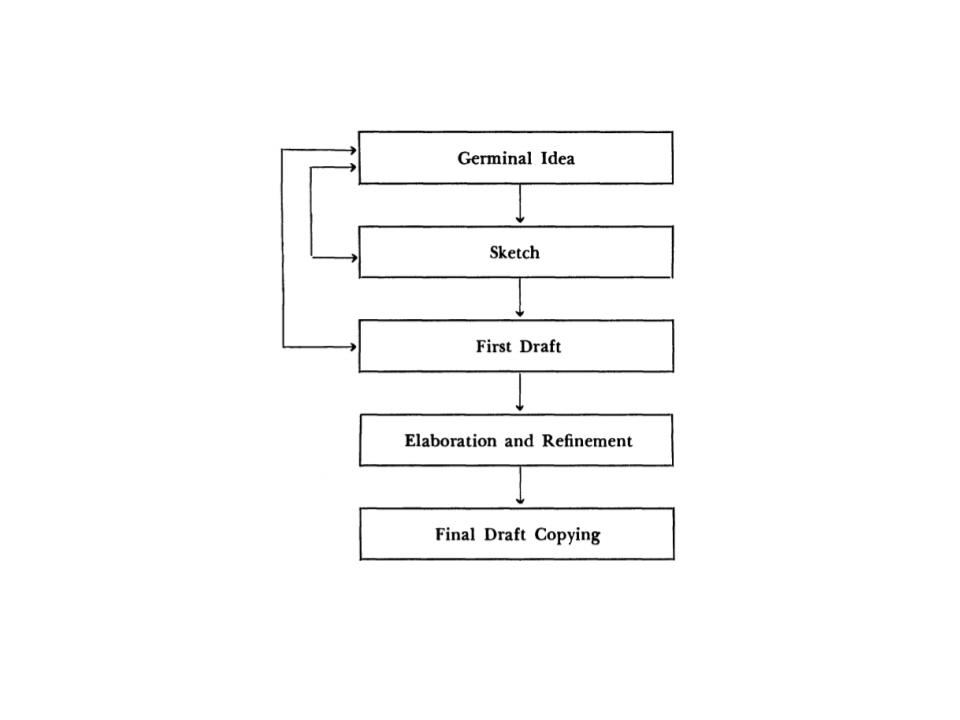
\includegraphics[width=12cm ]{figures/Composition.jpg}
    \caption{Stages of Music Composition \protect\cite{bennett1976process}}
    \label{fig:composition}
\end{figure}

\subsection{Music Fundamentals}
Music as defined in the study of \citeA{willoughby1971comprehensive}, is formed by combining the fundamentals of music. These fundamentals of music are discussed by \citeA{rivadelo1986fundamentals}. The author named the fundamentals as: rhythm, pitch, melody, texture and harmony, color and timbre, and form. 

In a composition, a sound can have a high or low tone which is related to the amount of vibrations per second, this is called pitch \cite{rivadelo1986fundamentals}. Pitches are represented by the first seven letters in the alphabet, namely A, B, C, D, E, F, and G \cite{miller2005complete}. The distances between a pitch from each other is illustrated as whole step, a half step, or semitone. In the keys of a piano or keyboard, moving from one key to a next key is called a half step or semitone respectively. A whole step was then described by \citeauthor{rivadelo1986fundamentals} as moving from one key to another and skipping the key between them. When adding the word up or down after the distance, half step, and whole step can traverse forward or backward. It is also possible to put a number before the distance in order to indicate multiple steps. 

Rhythm, as explained by \citeA{rivadelo1986fundamentals}, is made up of five distinguishable parts namely: clap, accent, meter, rhythmic pattern, and phrase. The clap is the key time unit used by the composition. The meter divides the claps into multiple sections. The accent is responsible for the formation of the theme of the rhythm. And lastly, the phrase is part of a musical thought, which is a component of the musical sentence.

Rhythm, as part of a composition, represents how fast or how slow the musical flow through the common patterns \cite{rivadelo1986fundamentals}. It is also understood that rhythm is the aspect that makes people aware of the tempo of the composition. It lets them adjust the ideas they have in order to add pitch and melody on top of the rhythm.

Another important component of a composition is the duration, which is basically the amount of time a tone or sound lasts \cite{rivadelo1986fundamentals}. This is seen in a composition in a staff through a note or rest. The type of note or rest indicates how long the duration of the pitch \cite{rivadelo1986fundamentals}. 

It is also important to note that rhythm depends on the tempo of the composition. The tempo defines the pace of the composition \cite{rivadelo1986fundamentals, nelson2009foundations}. Tempo is used by composers to set a mood or make the music more playable. Recently however, composers tend to use beats per minute to represent the tempo of a composition \cite{nelson2009foundations}.

There are seven common tempo markings according to \citeauthor{nelson2009foundations}. 
\begin{itemize}
    \item Grave, a very slow tempo. It has a bpm of around 25-40.
    \item Largo, a broad tempo. It has a bpm of around 40-60.
    \item Larghetto which is like largo but faster. It has a bpm of around 60-66.
    \item Adagio, a slow tempo but with great expression. It has a bpm of around 66-76.
    \item Andante, a walking pace tempo. It has a bpm of around 76-108.
    \item Moderato, a moderate speed tempo. It has a bpm of around 108-120.
    \item Allegro, a fast tempo it is also bright and quick. It has a bpm of around 120-156. 
\end{itemize}

FireflyX will be using these seven tempo markings to indicate the current tempo of the composition. The floor bpm of the tempo markings will be used to scale the speed of the composition.

\subsection{Musical Notation}
Musical notation is the method of visually representing musical sound \cite{read1964music}. Musicians use the notations to illustrate their musical ideas. As explained by \citeA{read1964music}, for people to be musically literate they would need to have an understanding of the symbols used in musical notation.

\begin{figure}[H]
    \centering
    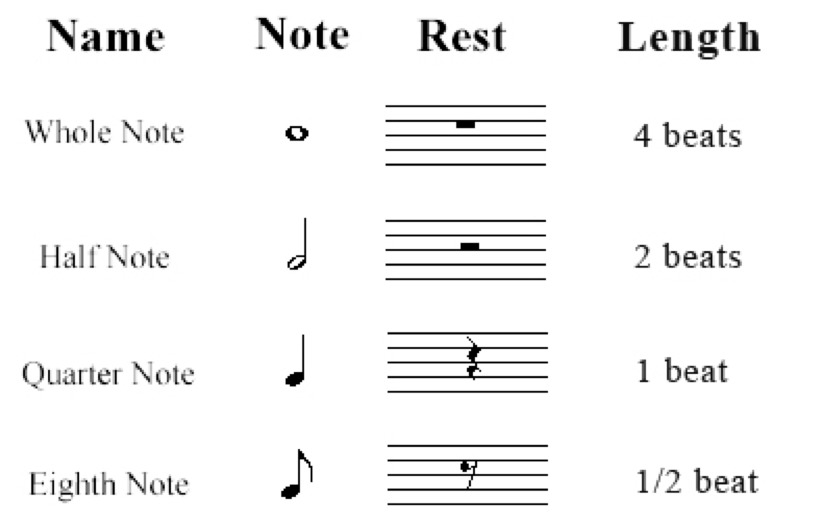
\includegraphics[width=10cm ]{figures/BasicMusicNotes.png}
    \caption{Basic notes and rests used in modern musical notation \protect\cite{BasicNotes2016}}
    \label{fig:BasicNotes2016}
\end{figure}

The notes and rests found in Figure \ref{fig:BasicNotes2016} are some of the basic symbols in musical notation. The symbol of the notes and rests represent how long a clap is. They staff is a set of lines and spaces which indicate the levels of pitches. The notes and rests are found throughout the staff, and their position on the staff represent their pitch. However, these pitches are also based on the clef found at the start of the staff. The G-clef as seen in figure \ref{fig:G-Clef} change the pitch represented by the staff. When it is used at the start of the staff, each line of the staff starting from the bottom represent the pitches E-G-B-D-F and the spaces represent the pitches F-A-C-E.

\begin{figure}[H]
    \centering
    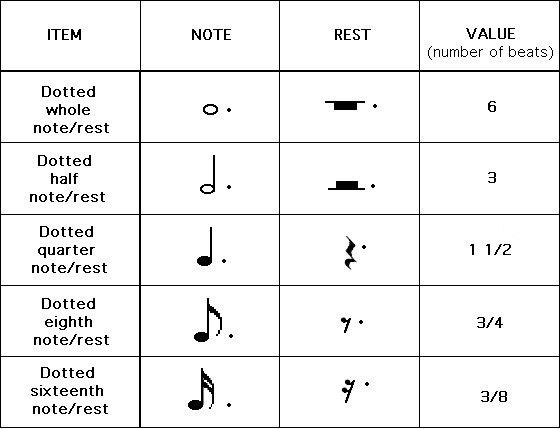
\includegraphics[width=10cm ]{figures/dotted_notes_chart.jpg}
    \caption{Dotted notations \protect\cite{DottedNotes2015}}
    \label{fig:DottedNotes2015}
\end{figure}

In addition to this, the duration of the note could be extended by putting a dot after the note. When a dot is added to the note, the duration of the note is increased by half of its original value. Multiple dots could be added and the subsequent dots add the progressively halved value. Examples of dotted notations and their equivalent duration can be found in Figure \ref{fig:DottedNotes2015}.

\begin{figure}[H]
    \centering
    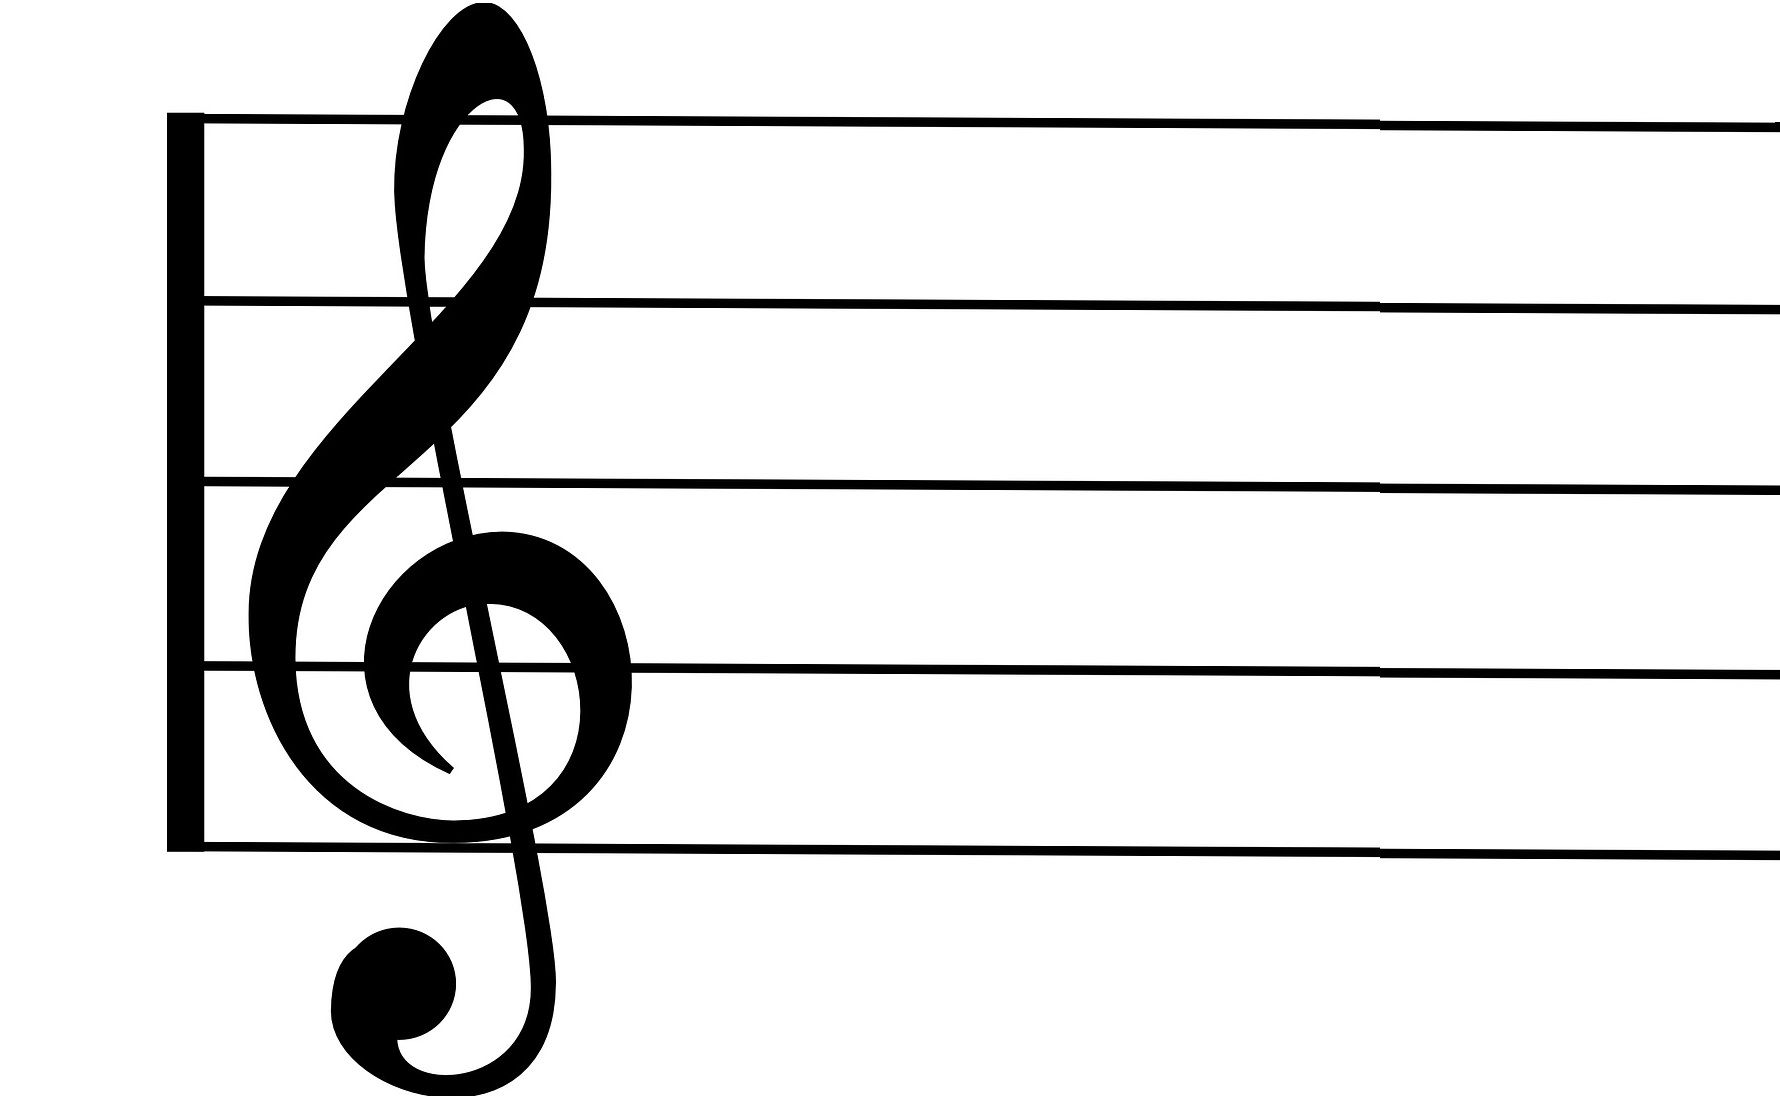
\includegraphics[width=5cm ]{figures/G-clef.jpg}
    \caption{The G-Clef \protect\cite{G-Clef}}
    \label{fig:G-Clef}
\end{figure}

The time signature defines the distinct rhythm throughout the composition \cite{rivadelo1986fundamentals}. As seen in figure \ref{fig:Time-Signature}, there are two numbers found in a time signature namely, the numerator and the denominator. In the time signature, the numerator always takes two spaces of the staff \cite{read1964music, rivadelo1986fundamentals, burrows1999read}.

\begin{figure}[H]
    \centering
    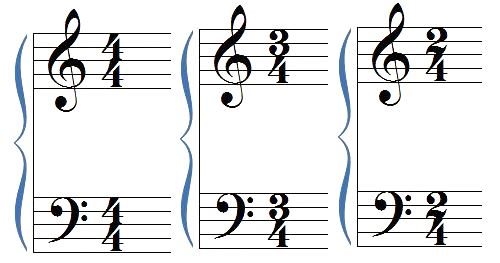
\includegraphics[width=7cm ]{figures/Time-Signature.jpg}
    \caption{The various time signatures \protect\cite{Time-Signature}}
    \label{fig:Time-Signature}
\end{figure}

The bar lines, as seen in figure \ref{fig:Bar-Lines} represent the division of notes in a musical sheet. There are two kinds of bar lines in musical compositions. The first kind of bar line is one vertical line that divides the notes based on the time signature of the staff. The second kind of bar line is the double bar line which is represented by two vertical lines. The double bar line is seen at the end of a composition \cite{read1964music}.  

\begin{figure}[H]
    \centering
    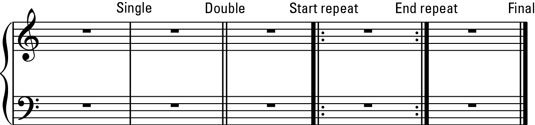
\includegraphics[width=9cm ]{figures/Bar-Lines.jpg}
    \caption{The various bar line notations \protect\cite{Bar-Lines}}
    \label{fig:Bar-Lines}
\end{figure}

\subsection{Music Language Synthesis}
Computer tools have recently been made to help in representing different elements of music, as natural languages are being made to help in representing the demands of music composition which will help in understanding music \cite{loy1985programming}.
\newline

One study aimed in making an open-ended programming language is the study of \citeA{dannenberg1997machine} named Nyquist. The study aimed to help in creating compositional tasks. By using Nyquist, sounds can be assigned into variables, stored into data structures, and can also be passed as parameters \cite{dannenberg1997machine}. In the study, musical composition can be represented as a series of sounds in a sequence and can be given arbitrary offsets. 

In Nyquist, expressions are written using Lisp \cite{turetsky1984lisp}, where parentheses define when applying a function to a set of parameters. An expression consists of variables and keywords. An example of an expression is seen in the expression \ref{NyquistExpression} where it simulates two notes. A reference of their keywords and representations could be seen in Table \ref{NyquistKeywords}.

\begin{equation}
          (sim (fminst\: g4\: 100) \\
        (fminst\: g4\: 100))
    \label{NyquistExpression}
\end{equation}


\begin{table}[H]
\centering
\label{NyquistKeywords}
\caption{Related Studies on Sandbox Environments and other Dynamic Interfaces \cite{dannenberg1997machine}}
\begin{tabular}{|l|l|} 
\hline
\textbf{Keyword in Nyquist}  & \textbf{Representation}                \\ 
\hline
defun                        & define function                        \\ 
\hline
at s t                       & shift sound s by t seconds in time     \\ 
\hline
seq                          & arranges sound sequentially            \\ 
\hline
sim                          & arranges sound simultaneously          \\ 
\hline
scale                        & scales sound to a different amplitude  \\ 
\hline
play                         & plays the sound                        \\ 
\hline
fminst                       & pitch depth                            \\
\hline
\end{tabular}
\end{table}

A thesis by \citeA{ince2019programming} also emphasized in the use of patterns in representing music as they described them as events in time. Where these structures of music can be formed into a sequence of events, as this idea is used in specifying the music pattern in a language. Their application named Siren emphasizes on the creation of these patterns as they found inspiration from Haskell a pattern language, which generates a \say{library of patterns} to represent music \cite{ince2019programming}.

FireflyX will be implementing clap-rest patterns that will represent the parts of the firefly model. Techniques in the work of Nyquist specifically music as a set of parameters will be implemented for the program to read the configuration from an XML file. The configuration will then be parsed by a playback module and produce sound.


% The goal of Nyquist is to
% provide an open-ended programming language that
% supports high-level compositional tasks in addition
% to low-level signal processing.
% Sounds are first-class types in Nyquist;
% hence they can be assigned to variables, passed as
% parameters, and stored in data structures.
% Composition requires that sounds be placed simultaneously, in sequence, and at arbitrary offsets.

% For example, the expression
% (osc c4)
% means "apply the function osc to the parameter
% c4." Parameters are evaluated first. In this case, c4
% is a global variable (intended to remain constant)
% containing the value 60.0. The value 60.0 is passed
% to the osc function, and the result is a sinusoid
% whose frequency corresponds to middle C and
% whose duration is 1 sec.



%\section{Children's Learning}

%The early years in a child's life are important for learning. It is because learning is dependent on the plasticity of the brain which is strongest in those early years. This learning can stimulate brain growth and improve fine motor coordination \cite{gruhn2005children}. Learning on its own happens without people's consciousness. When listening to music, people process a lot of information.\cite{hallam2010power} These processed information leads to possible improvement in different fields such as mathematics, reading, and IQ in general \cite{vcrnvcec2006cognitive}. 
%
%A study by \cite{leung2010students} mentions that in Hong Kong, the music curriculum is aimed to teach students to develop in certain fields. One field to be developed is creativity and imagination. Another is the aim to develop skills and processes. Both of these can be developed by direct musical activities such as instrument playing and singing. During this process of learning, students are encouraged to act independently as they solve musical challenges so that one day they may become confident in solving problems in their daily lives.
%challenges
%Studies suggest however that even with its benefits, there are some challenges that come with it. One study \citeauthor{russell2009me} mentions of different things that public schools in order to teach music properly. The lack of knowledge, time, priority, experience, and resources are the main causes of public schools being unable to teach music properly. Teachers with the lack of knowledge of syllabus requirements and the lack of personal experience make them unable to teach properly. This also goes for the lack of time to prepare and to teach making the music lesson lacking.  The is usually also caused by the school not giving musical lessons any priority which also leads to the lack of resources to teach music with. 
%
%Another study by \citeauthor{may2013public}, mentions that the teachers must optimize the class environment for the music classes. For children, play is primary means of education as it something they are motivated to do on their own. A good music classroom would be one with an array of instruments for children to play with and explore.


%
%Interaction Design


% \section{User Research}
% \subsection{Experiment Design}


